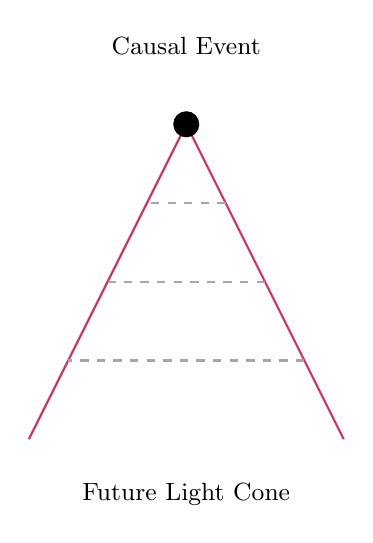
\begin{tikzpicture}[
    cone/.style={draw=purple!80, thick},
    slice/.style={draw=gray!70, dashed, thick},
    event/.style={circle, fill=black, minimum size=5pt},
]

% Future cone
\draw[cone] (0,0) -- (-2,-4);
\draw[cone] (0,0) -- (2,-4);

% Slices
\foreach \y in {-1,-2,-3}{
  \draw[slice] (-2*\y/4,\y) -- (2*\y/4,\y);
}

\node[event] at (0,0) {};

\node at (0,1) {\small Causal Event};
\node at (0,-4.7) {\small Future Light Cone};

\end{tikzpicture}